\documentclass{article}
\title{Synthetic Sympatric Speciation Through Meiotic Inheritance}
\author{William Booker - Version 2.08}
\date{February 16, 2017}

\usepackage[utf8]{inputenc}
\usepackage{natbib}
\usepackage{graphicx}
\usepackage{subcaption}
\usepackage{xcolor}
\newcommand\TODO[1]{\textcolor{red}{#1}}



\begin{document}
\maketitle

%\TODO{GET GRAPHS IN THE RIGHT PLACE}
%\TODO{ADD ADDITIONAL CITATIONS}
%\TODO{CHECK TENSE CHANGES?}

\section{Abstract}

Speciation is a critical process for both evolutionary science and machine learning. It helps us understand the development of life on Earth and can improve genetic algorithms' ability to find global maximums. In recent years, there has been considerable effort to understand this elusive process and uncover new techniques to simulate it. While there are many approaches for doing so, few examine one of the most important features of any genetic system: inheritance. This paper seeks to address this shortcoming and demonstrate how minor changes to a population's inheritnace mechanism can radically alter a it's ability to speciate. Specifically, we look at how simulated meiotic inheritance with complete gene dominance can significantly improve a population's divergent capability, even in absance of other speciation pressures. 



\section{Introduction}

Speciation describes the natural tendancy for homogenous populations to split and form discrete groups through the continuous process of evolution. \cite{SPBOOK} It underpins our understanding of biology and it is fundamental to the development of life on this planet. Additionally, speciation shows promise in the realm of artificial intelligence, as a mechanism by which to narrow in on optimal solutions in multi-modal solution spaces.

Evolutionary biologists define two distinct types of speciation: allopatric speciation, where isolated populations acquire new traits independently, and sympatric speciation, where a single population diverges over time. For our purposes, we are mostly concerned with sympatric speciation, as it has the most potential to improve genetic algorithms. While there are many methods for inducing a type of allopatric speciation in genetic algorithms, such as such as niching \cite{NICHING}, population topologies \cite{TOPOLOGIES}, and island models \cite{ISLAND}, these approaches require implicit assumptions about the solution space which must be explicitly tailored to each problem. Ideally we would like to find a more general solution, where the algorithm speciates correctly in a number of different enviornments. 

For our experiments in sympatric speciation, we chose to examine an evolutionary model designed my Mark Woener et al. as part of the paper \textit{Sexual Selection, Resource Distribution, and Population Size in Synthetic Sympatric Speciation}. In the paper, the researchers hypothesized that sexual selection may be key to inducing sympatric speciation, as it has the potential to isolate sub-groups within a population, which could then evolve different traits in a similar manner to allotropic speciation. To test this hypothesis, the researchers set up a 2x2 factorial study using a simulated population of finches. In the study, the researches created two different distributions of seeds, bimodal and uniform, and observed the differences in population dynamics between finches that utilized sexual selection and those that did not.

While the researches successfully demonstrated that sexual selection was an effective method to induce sympatric speciation in a population, some of the results in their control study seemed to contradict our understanding of biological speciation. Specifically, when a population without sexual selection encountered a bimodal seed distribution, the population never expanded to cover both possible niches. This result is peculiar, as any species is highly incentivized to take advantage of all available niches in its environment. The convergence exhibited in the bimodal seed random mating scenario is known as bottlenecking, and typically only occurs in small, declining populations \cite{CHICKEN}. To see bottlenecking occurring in a large, healthy population suggests that there is another factor at play, which enables more phylogenetic divergance in biological populations.



\section{Hypothesis}

The cause of the population convergence in the bimodal seed random mating scenario is due to an oversimplification of genetic inheritance. Averaging the beak-sizes of the parents inhibits a population’s ability to maintain genetic diversity, which leads to population collapse in multi-niche environments. A more biologically accurate simulation employing a form of meiotic inheritance would exploit both niches in the BSRM scenario.



\section{Methods}

This research consisted of five experiments: three primary experiments and two supplemental experiments. The three primary experiments are designed to test our hypothesis that the introduction of meiotic inheritance radically changes the behavior of the system. The two supplemental experiments are designed to help us better understand why those changes arise. 



\subsection{Experiment 1 -- Replicating Results}

The initial simulation is designed to replicate the simulation from the \textit{Speciation} paper. The details of this simulation are summarized in the following paragraphs. For a more in-depth analysis on the reasoning behind the choices made, please consult the original paper. 

The simulation consists of an island 100x100 units in size, filled with seeds and inhabited by a population of finches. Each finch has a known beak-size, age, gender, energy-level, and location. Each seed has a known size, energy-level and location.

The simulation begins by generating 400 finches with a roughly equal number of males and females. This initial population has a mean beak-size of  5.5 and a standard deviation of 0.5 \footnote{The \textit{Speciation} paper actually specifies a variance of 0.5, but the their data suggest that they actually used a standard deviation of 0.5.} (Gaussian distribution). These finches have their energy level set to zero and are randomly spread around the island. The island then undergoes an annual cycle consisting of a dry season and a mating season. This cycle repeats 1000 times during the simulation. 

The dry season lasts 100 days, and begins by spreading 5000 seeds randomly around the island. Each day, each bird has a chance to forage for food. The foraging is performed in a random order. Each bird searches a 10x10 plot of the island and consumes the first seed it finds that falls within one unit of its beak-size. This search costs the finch 0.1 units of energy. Any finch that has less than zero units of energy at the end of the day is declared dead and removed from the population.

The simulation accounts for two different distributions of seed sizes: bimodal and uniform. The bimodal distribution consists of two Gaussian distributions of 2500 seeds each; these distributions are centered at three and eight units, each with a standard deviation of 0.5 units. The uniform distribution consists of a single uniform distribution of 5000 seeds ranging from one to ten units in size. In both scenarios, a seed contains between zero and two units of energy (uniform distribution).

After the dry season ends, the remaining finches participate in that year's mating season. During the mating season, each female chooses a single male to mate with. The simulation accounts for two types of mating: random mating, where females will choose any male from the population, and assorted mating, where females will only pick males within one unit of its beak-size. Each male is only allowed to mate with five females per year. When presented with multiple possible mates, the female will choose between them at random. Mating produces a single offspring at the location of the mother. The child’s beak-size is an average of the beak-sizes of the parents plus a small Gaussian-random mutation (mean 0, standard deviation 0.2).

This process results in four discrete cases: bimodal seeds assorted mating (BSAM), bimodal seeds random mating (BSRM), uniform seeds assorted mating (USAM), and uniform seeds random mating (USRM). Each case is replicated 48 times to ensure accurate results and to give insight into population extinction rates. 



\subsection{Experiment 2 -- Introduction of Genetic Structure}

The objective of this experiment is to replace the simplistic inheritance structure with a more robust genetic model while still maintaining the averaging process. This step serves as a control study to demonstrate that the changes in the third experiment are a result of the introduction of meiotic inheritance rather than the introduction of the new genetic structure. This genetic structure is designed to mimic genes in the natural world as closely as possible.

Each finch is equipped with two sets of genes, one from each parent. Each gene contains an array of one-hundred sub-genes, each represented by a floating point value. The phenotype for a gene is determined by taking the sum of all of the sub-genes. In order to mimic the \textit{Speciation} paper’s initial population, the sub-genes in the initial population are randomly chosen from a uniform distribution with a mean of 0.055 and a range of 0.245 \footnote{The mean of 0.055 and the range of 0.245 were determined mathematically. The final beak-size is equal to the average of two sums of 100 sub-genes, or $(\sum_{i=1}^{200} x_{i})/2$. The distribution of the beak-sizes is normal by the central limit theorem. The mean is $(200 * 0.055)/2 = 5.5$, and the standard deviation is $\sqrt{\frac{1}{4}\sum_{i=1}^{200}Var(x_{i})} = 0.5$ where $Var(x_{i}) = \frac{0.245^2}{12}$.}. A single gene was used to determine the beak-size of the individual. This choice reflects how a single gene, Bmp4, is responsible for most of the variation in beak-sizes in real Darwinian finches \cite{BMP4}. 

Our experiments use both a complete dominance and an incomplete dominance model. In the complete dominance model, the larger of the two phenotypes is chosen for the finch's beak-size. In the incomplete dominance model, the two phenotypes are averaged to determine the beak-size. Note that for the purposes of inheritance this choice is arbitrary, as neither model affects the actual genetic material that is passed on to the child. 

In order to maintain the averaging process, when mating, the sub-genes of each parent are averaged to determine the sub-genes for the child. Each sub-gene has a 10\% chance to mutate after the averaging process. When a sub-gene is selected for mutation, we add a random value taken from a uniform distribution with a range of 0.310 and a mean of 0 \footnote{The running mutation range of 0.310 was determined empirically. We iteratively tested mutation ranges until the standard deviation of the change in beak-size consistently averaged at 0.2}.


	
\subsection{Experiment 3 -- Introduction of Meiotic
Inheritance}

The setup for the third experiment is nearly identical to that of the second: the only change is the addition of meiotic inheritance. During mating, rather than average the sub-genes of the parent's genes, the child receives one randomly selected gene from each of its parents. The mutation rate and range remain the same as in the previous step. 



\subsection{Experiments 4-5 Notes}

In the fourth and fifth experiments, we made two major changes when compared to the initial three experiments. First, rather than testing all population conditions, we only looked at the meiotic population conditions and one non-meiotic population condition in the BSRM scenario. Second, we reduced the initial population size from 400 down to 40 to help smooth out the initial population collapse and subsequent rebound that appeared in our first three experiments.

\subsection{Experiment 4 -- Removing Mutation}

The fourth experiment is designed to illustrate the convergent tendency of the averaging inheritance method by removing the noise caused by mutation. We achieved this effect by reducing the range of the running mutation rate from 0.310 to 0.00. We also quadrupled the initial mutation rate to 0.980 in order to give the starting population sufficient diversity to reach both niches. 

\subsection{Experiment 5 -- Modifying The Initial Population}

The fifth experiment is a response to an unexpected result in our third experiment, where complete dominance exhibited far higher speciation rates than incomplete dominance. In this experiment, we changed the size of the initial population to see the effects on the relative extinction rates between incomplete dominance and complete dominance. For the first test, we widened the initial population by quadrupling the mutation rate to 0.980. In the second test, we reduced the initial population by halving the mutation rate to 0.1225 and moving the mean to 0.80. This change centers the population in the middle of the upper niche.



\section{Results}

The results of our experiments are given in the form of population trees and extinction rates. The trees are organized into tables such that the columns represent gene structures and the rows represent the seed distributions and mating types.

\subsection{Experiments 1-2 -- Replication and Gene Structure}

The results from the first two experiments are given in figure \ref{fig:EXP2} and table \ref{table:EXP2}. In figure \ref{fig:EXP2}, the first column represents our replication of the \textit{Speciation} paper's results, while the second and third columns represent the introduction of the new genetic structure. The results from the first experiment closely match the results of the \textit{Speciation} paper. As expected, we see high rates of speciation in the BSAM and the USAM scenarios and no speciation in the BSRM and the USRM scenarios. The population trees and extinction rates from the second and third experiment closely match those from the first, indicating that the introduction of the genetic structure had little impact on the results of the simulation.

\begin{figure} [h!]
    \centering
    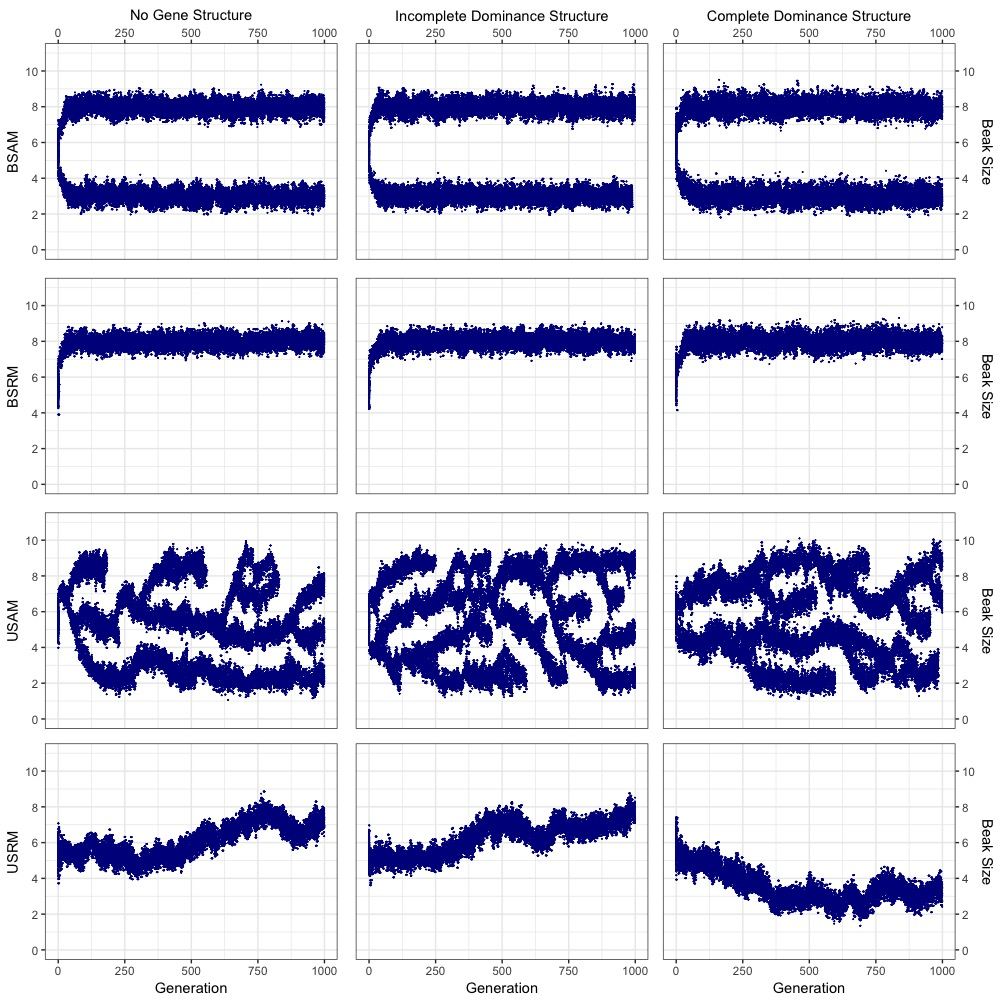
\includegraphics[width=\linewidth]{Data/EXP2}
    \caption{Introduction of Gene Structure}
    \label{fig:EXP2}
\end{figure}

\begin{table} [ht!]
\centering
    \begin{tabular}{| p{2.75cm} *{4}{|c} |}
        \hline
        BSAM & Baseline & Replication & Avg Idom & Avg Cdom \\ \hline
        Speciation & 31 & 30 & 25 & 23 \\ \hline
        Partial Extinction & 17 & 15 & 23 & 21 \\ \hline
        Extinction & 0 & 3 & 0 & 4 \\ \hline
    \end{tabular}
    \begin{tabular}{| p{2.75cm} *{4}{|c} |}
        \hline
        BSRM & Baseline & Replication & Avg Idom & Avg Cdom \\ \hline
        Speciation & 0 & 0 & 0 & 0 \\ \hline
        Partial Extinction & 41 & 38 & 35 & 35 \\ \hline
        Extinction & 7 & 10 & 13 & 13 \\ \hline
    \end{tabular}
    \begin{tabular}{| p{2.75cm} *{4}{|c} |}
        \hline
        USAM & Baseline & Replication & Avg Idom & Avg Cdom \\ \hline
        Speciation & 35 & 37 & 41 & 41 \\ \hline
        Extinction & 13 & 11 & 7 & 7 \\ \hline
    \end{tabular}
    \begin{tabular}{| p{2.75cm} *{4}{|c} |}
        \hline
        USRM & Baseline & Replication & Avg Idom & Avg Cdom \\ \hline
        Single Species & 35 & 23 & 24 & 34\\ \hline
        Extinction & 13 & 25 & 24 & 14 \\ \hline
    \end{tabular}
    \caption{Replication and Gene Structure}
    \label{table:EXP2}
\end{table}



\subsection{Experiment 3 -- Introduction of Meiotic Inheritance}

The results from the third experiment are given in figure \ref{fig:EXP3} and table \ref{table:EXP3}. The first column of figure \ref{fig:EXP3} is equivalent the incomplete dominance scenario from the second column of figure \ref{fig:EXP2}. Columns two and three represent the introduction of meiotic inheritance. As the data shows, the introduction of meiotic inheritance radically altered the behavior of each of the population. Specifically, it broadened the population bands, and occasionally induced speciation in the BSRM scenarios. Note that these speciation events occur far more frequently in the complete dominance structure than in the incomplete dominance structure.

\begin{figure} [ht!]
    \centering
    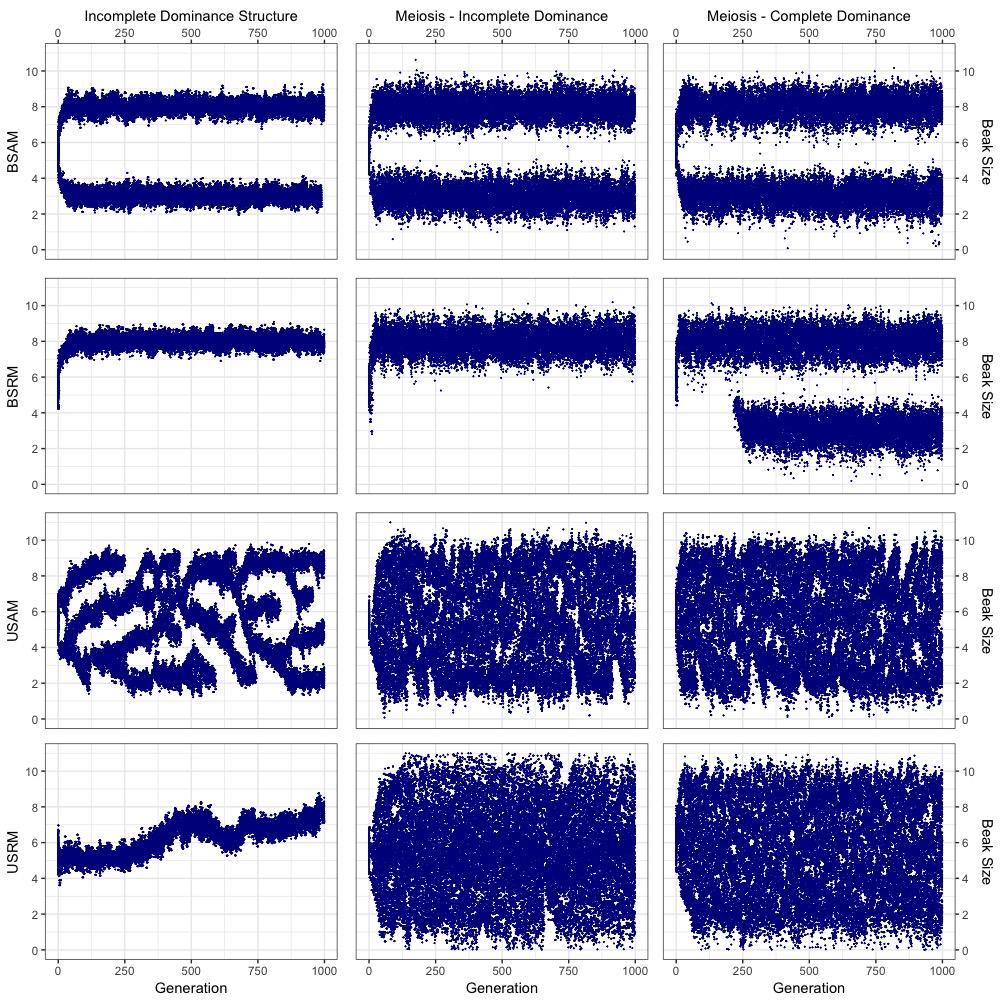
\includegraphics[width=\linewidth]{Data/EXP3}
    \caption{Introduction of Meiotic Inheritance}
    \label{fig:EXP3}
\end{figure}

\begin{table} [hb!]
\centering
    \begin{tabular}{| p{2.75cm} *{3}{|c} |}
        \hline
        BSAM & Avg Idom & Meiosis Idom & Meiosis Cdom \\ \hline
        Speciation & 25 & 31 & 20 \\ \hline
        Partial Extinction & 23 & 15 & 27 \\ \hline
        Extinction & 0 & 2 & 1 \\ \hline
    \end{tabular}
    \begin{tabular}{| p{2.75cm} *{4}{|c} |}
        \hline
        BSRM & Avg Idom & Meiosis Idom & Meiosis Cdom \\ \hline
        Speciation & 0 & 1 & 33 \\ \hline
        Partial Extinction & 35 & 30 & 14 \\ \hline
        Extinction & 13 & 17 & 1 \\ \hline
    \end{tabular}
    \begin{tabular}{| p{2.75cm} *{4}{|c} |}
        \hline
        USAM & Avg Idom & Meiosis Idom & Meiosis Cdom \\ \hline
        Speciation & 41 & 37 & 41 \\ \hline
        Extinction & 7 & 11 & 7 \\ \hline
    \end{tabular}
    \begin{tabular}{| p{2.75cm} *{4}{|c} |}
        \hline
        USRM & Avg Idom & Meiosis Idom & Meiosis Cdom \\ \hline
        Single Species & 24 & 44 & 40 \\ \hline
        Extinction & 24 & 4 & 8 \\ \hline
    \end{tabular}
    \caption{Introduction of Meiotic Inheritance}
    \label{table:EXP3}
\end{table}



\subsection{Experiment 4 -- Removing Mutation}

The results of the fourth experiment are given in figure \ref{fig:EXP4} and represent the difference between averaging and meiotic inheritance in the absence of mutation. Both simulations utilize an incomplete dominance genetic structure. As expected, the non-meiotic population exhibited clear signs of convergence, while the meiotic population retained population diversity throughout the duration of the simulation. 

\begin{figure} [ht!]
    \centering
    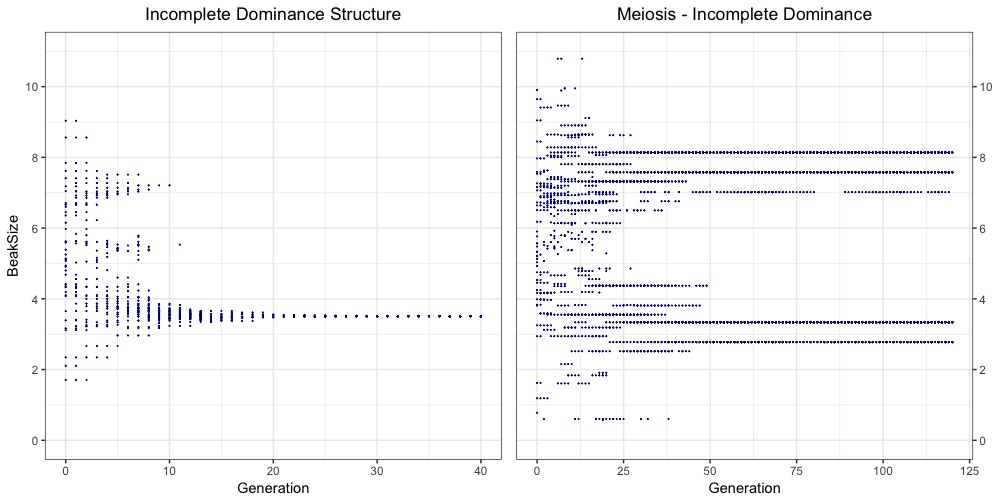
\includegraphics[width=\linewidth]{Data/EXP4}
    \caption{Removed Mutation}
    \label{fig:EXP4}
\end{figure}



\subsection{Experiment 5 -- Modifying The Initial Population} 

The results of the fifth experiment are given in figure \ref{fig:EXP5} and table \ref{table:EXP5}. The first column of figure \ref{fig:EXP5} represents the incomplete dominance case with the averaging inheritance method. The second and third columns represent meiotic inheritance with incomplete and complete dominance. When the population was widened, both meiotic populations exhibited high rates of speciation. When the population was narrowed, only the complete dominance case speciated, and the rate of specition was drastically reduced. The non-meiotic population exhibited no speciation events in either scenario. 

\begin{figure} [ht!]
    \centering
    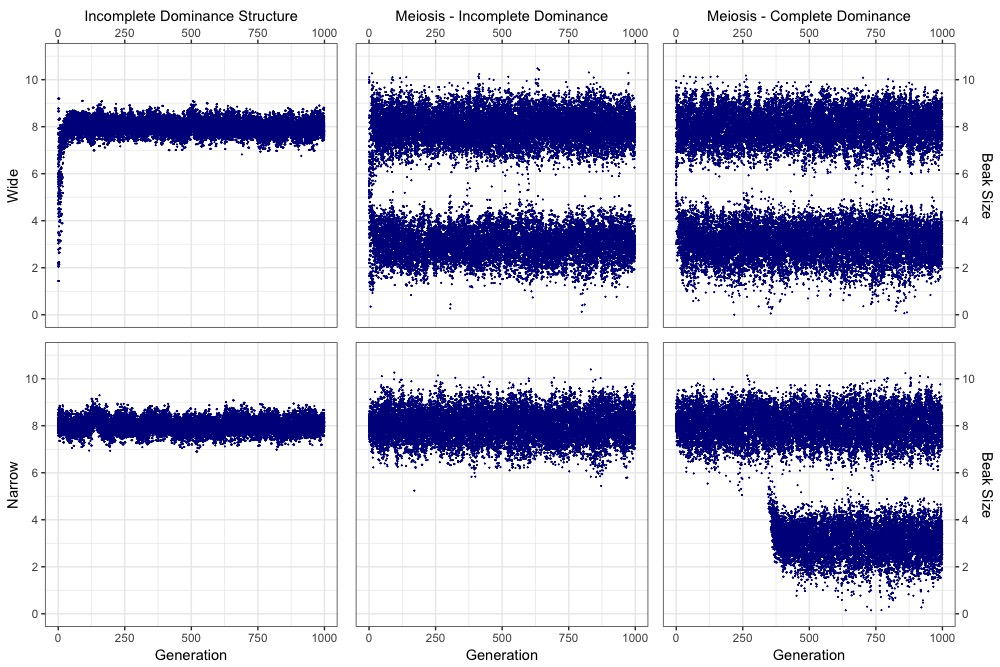
\includegraphics[width=\linewidth]{Data/EXP5}
    \caption{BSRM Scenario with Varying Initial Populations}
    \label{fig:EXP5}
\end{figure}

\begin{table} [htbp]
\centering
    \begin{tabular}{| p{2.75cm} *{3}{|c} |}
        \hline
        Wide & Avg Idom & Meiosis Idom & Meiosis Cdom \\ \hline
        Speciation & 0 & 39 & 43 \\ \hline
        Partial Extinction & 45 & 9 & 5 \\ \hline
        Extinction & 3 & 0 & 0 \\ \hline
    \end{tabular}
    \begin{tabular}{| p{2.75cm} *{3}{|c} |}
        \hline
        Narrow & Avg Idom & Meiosis Idom & Meiosis Cdom \\ \hline
        Speciation & 0 & 0 & 12 \\ \hline
        Partial Extinction & 46 & 48 & 33 \\ \hline
        Extinction & 2 & 0 & 3 \\ \hline
    \end{tabular}
    \caption{BSRM Scenario with Varying Initial Populations}
    \label{table:EXP5}
\end{table}



\section{Analysis}

In our first experiment, we were largely successful in replicating the results from the \textit{Speciation} paper. In the BSAM, BSRM, and USAM cases, the population distributions, the widths of the population bands, and the number of extinction events lined up extremely well with what was described in the \textit{Speciation} paper. In the USRM scenario, the population distribution and the widths of the bands were correct, but there were significantly more extinction events than expected. We suspect that this anomaly might be due to a minor difference between our implementation and that of the initial experiment that was not covered in the original paper. Furthermore, it’s worth noting that we experienced another anomaly in the USRM scenario in the second experiment, suggesting that the extinction rates in this scenario might be unusually sensitive to minor changes in experimental setup. However, barring this anomaly, we are confident that we have successfully replicated the \textit{Speciation} paper’s results. 

In the second experiment, we introduced the new genetic structure but kept the averaging method the same, then compared the results against our findings from the first experiment. As expected, the population trees and extinction rates closely matched our original results. Again, the only major variation was in the extinction rates for the complete dominance structure in the USRM scenario. We suspect that this variation may have been the result of the slight skewing of the phenotypes of the initial population, caused by the switch from incomplete dominance to complete dominance. Nevertheless, this experiment demonstrates that the new genetic structure had little impact on the behavior of the populations.

In the third experiment, we used the same genetic structure as the second experiment with the addition of meiotic inheritance. This change radically altered the result of the simulation. Rather than collapsing into narrow bands, each population rapidly expanded to cover the entire range of seed sizes. These extremely thick population bands indicate that the meiotic populations exhibited far more genetic diversity than the non-meiotic populations. Furthermore, unlike the non-meiotic populations, the meiotic populations exhibited evidence of speciation in the BSRM scenario. This observation contradicts the results from the initial \textit{Speciation} paper, where the researchers demonstrated that sexual selection was requisite for sympatric speciation. The key to this discrepancy lies in the mechanism by which genes are passed on to the next generation. 

In the original experiment, we average the beak-sizes of the parents to determine the beak-size of the child. While seemingly sensible, this approach destroys important genetic diversity in the population. Barring mutation, any child produced using this method will have a beak-size between the beak-sizes of its parents. When scaled up, this effect causes each generation to cover a smaller range of beak-sizes than the generation that preceded it. Thus, over time, the species begins to coalesce around a single beak-size: population convergence. As the inheritance method pushes the population inwards, the high mutation rate pushes the population outwards, eventually reaching equilibrium at two-unit thick population bands. This equilibrium is why the size of the population bands are the same with regardless of niche size: the inheritance method is the force pushing the population inwards, not natural selection. This effect also explains why we don’t see speciation in the BSRM scenario for non-meiotic populations. Because the gap between the local maxima at three and eight are more than two units apart, there is no stable population that can contain both, forcing one niche to be abandoned.

Contrast this tendency with non-destructive meiotic inheritance, in which genetic information is passed unaltered from parent to child. By keeping the genes the same between generations, meiotic inheritance protects the diversity of the population. There is no guarantee that a child’s beak-size will fall between that of its parents, so future populations can reassert genetic diversity that may not appear in the current distribution of phenotypes. By introducing meiotic inheritance in the third experiment, we removed the pressure towards convergence, allowing the population to diverge to cover the entire range of seed sizes. This change is why the population bands from the third experiment are so much wider than those of the first two: by removing the convergent inheritance method, the only factor restraining the population is the size of its niche. Furthermore, because meiotic populations have no tendency for convergence, and are thus stable at an arbitrary range, they can exploit both population niches in the BSRM scenario.

We observed these effects more clearly in our fourth experiment, where we removed the ability for the population to mutate over time. Without the divergent pressure from mutation, the averaging method immediately coalesced around a single beak-size. As predicted, each generation exhibited less diversity than the generation that proceeded it, eventually forcing the population to abandon one of the niches within a dozen generations. However, with meiotic inheritance, no such trend appeared. While some genes did die out, the handful of genes that survived were stable for the duration of the simulation. Some phenotypes even temporarily disappeared from the population, only to reemerge in later generations. These observations line up well with what we observe in real-world biological populations. Like the meiotic simulations, biological populations tend to exhibit a countable number of discrete phenotypes, and demonstrate high levels of diversity despite extremely low mutation rates [1]. While the simulated non-meiotic populations may look biologically accurate due to high mutation rates, this experiment demonstrates that they are actually governed by vastly different forces than biological populations, making them unreliable for predicting biological behavior. 

However, while we have illustrated why meiotic populations can exhibit speciation in the BSRM scenario, we have not addressed why complete dominance exhibited far higher rates of speciation than incomplete dominance. This effect is caused by an unrelated property of genetic inheritance, which we have termed \textit{gene masking}. Gene masking is a mechanism by which a population can bridge the evolutionary valley between the two optimums via genetic drift. In the case of complete dominance, only one gene is actually expressed, thus allowing the non-dominant gene to move through the low-fitness valley without reducing the organism’s evolutionary fitness. Eventually, these recessive genes can wander into the second niche, and, when matched, they produce an individual capable of exploiting these untapped resources. With incomplete dominance, both genes are expressed, so the population is unable to bridge the gap on its own. By masking the effect of one of the genes, complete dominance acts as a sort of multiplier on the mutation rate, allowing beneficial mutations to develop over the course of several generations rather than within a single individual.

Our fifth experiment was designed to test this analysis. Assuming that the change in speciation rates was due to the introduction of gene masking, we would expect that increasing the genetic diversity of the initial population would reduce its impact, while reducing the genetic diversity would increase it. Our results confirm this analysis. When the initial population was widened, incomplete dominance performed almost identically to complete dominance, with thirty-nine speciation events to forty-three. However, when the initial population was narrowed and confined to a single niche, there were no speciation events for incomplete dominance and twelve for complete dominance. Note that the averaging method did not produce any speciation events in either condition. These results suggest that both incomplete dominance and complete dominance are equally effective in protecting genetic diversity in a population; complete dominance only performed better in the third experiment because it added a method to bridge the low-fitness valley.



\section{Conclusion}

This research demonstrates the paramount importance of inheritance methods in biological simulations and genetic algorithms. A slight change in a population’s inheritance mechanism can radically alter the population dynamics, due to the potential introduction of strong evolutionary pressures. Obviously, for biological simulations, the inheritance process should mimic meiotic inheritance as closely as possible to avoid potential inaccuracy. While the applications for machine learning are less clear, we postulate that meiotic inheritance may have many advantages over assorted mating for inducing speciation in genetic algorithms.

First, meiotic speciation has an advantage in that it makes very few assumptions about the nature of the solution space. As demonstrated, destructive inheritance has a tendency to collapse into narrow population bands that are only sustained by high mutation rates. If the mutation rate is too low, these narrow population bands run the risk of getting stuck local maxima before they are able to identify the optimal solution. This observation reduces the generalizability of the sexual selection technique, as the mutation rate would likely have to be hand-crafted to optimize for a given solution space. Meiotic inheritance avoids this problem entirely by preventing population collapse during runtime. By keeping the population as wide as the niches will allow, meiotic inheritance is better protected against premature optimization.

Second, meiotic speciation has the potential to speed up the mating process, as random mating can be performed in O(n) time while sexual selection may take up to O($n^2$) time. Unlike with destructive inheritance, where sexual selection was requisite for speciation, in meiotic inheritance, sexual selection is unnecessary, and in some cases, even counter effective \footnote{In experiment 3, the speciation rate was higher in the BSRM complete dominance scenario than it was in the BSAM complete dominance scenario. This result stems from the fact that with assorted mating, the first member of new species is at a disadvantage, because its beak-size is too extreme to mate with the broader population.}. While it did not have a major impact on our simulation, if an algorithm wanted to have a high chance of finding the optimal solution by seeding a large portion of the problem space, this difference may improve performance. 

Third, meiotic speciation has the ability to take advantage of gene masking, which we discovered may be a powerful tool for exploring new niches without having to increase the mutation rate. This ability is advantageous, as increasing mutation rates often result in the accidental abandonment of good solutions \cite{TAGGING}. Meiotic inheritance is best equipped to utilize this technique, as the amount of genetic drift is not limited by the convergent tendency of the inheritance method.

Fourth, and perhaps most importantly, meiotic inheritance may prove useful in situations where the population space is evolving over time, potentially even in response to the genetic algorithm. In this case, it's easy to imagine how premature optimization may trap a population in a niche from which it is unable to escape once it becomes unfavorable. Meiotic inheritance would be well equipped to deal with such a scenario, given the high level of diversity and the ease with which it exploits new niches. When coupled with the additional search range offered by gene masking, meiotic inheritance gains a major advantage over sexual selection in dynamic solution topographies. 

Of course, there are some disadvantages to this technique. One issue is that our experiments use a dynamic population size, which, while biologically accurate, is uncommon in genetic algorithms. To expand the scope of this research, we would need to demonstrate an effective method by which to apply the benefits of meiotic inheritance onto a static population. Additionally, genetic algorithms that use an indirect encoding scheme often implicitly utilize a form of non-destructive inheritance, so there is little to be gained by altering these inheritance methods. Furthermore, in some applications convergent tendency is desired, as it can help to home in on a solution after the optimal peak has been identified. We hypothesize that the most effective inheritance method for solving multimodal problems likely begins with a non-destructive inheritance method and switches to a destructive inheritance method after identifying the major peaks. Thus, perhaps the most critical aspect of this research is that it demonstrates the importance of inheritance methods on populations, and illustrates the need for increased scrutiny of a rather under-appreciated aspect of genetic algorithms.

Finally, from a biological standpoint, it still remains to be seen how sexual selection impacts sympatric speciation in the natural world. While we have demonstrated that the \textit{Speciation} paper’s results cannot be applied to biological populations, we have not established whether or not sexual selection is a key component of biological sympatric speciation. Our results should not be haphazardly extended to the biological world, because the speciation that we observed in meiotic populations in the BSRM scenario is likely very different from the speciation exhibited in biological populations. Specifically, for the purposes of this paper, we defined speciation as any set of visibly distinct populations exploiting separate niches. However, while useful for genetic algorithms, this definition is weaker than biological speciation, which typically requires that different species be reproductively isolated \cite{TEXTBOOK}. Thus, it could be argued that the distinct bands that arise in meiotic populations in the BSRM scenario do not actually encompass two distinct species, but rather a single species exploiting multiple niches. Further research is required to determine if sexual selection is required for this split population to diverge into separate species, or if there is another potential cause.

In summary, the findings of this paper are fourfold. One, we successfully replicated the results of the \textit{Speciation} paper and confirmed their findings. Two, we demonstrated that meiotic inheritance radically changes the behavior of the simulation, thus providing evidence against the \textit{Speciation} paper's biological conclusions. Three, we demonstrated that non-destructive inheritance allows for speciation in multi-niche environments, which may have applications in genetic algorithms. And four, we demonstrated that gene masking gives populations the opportunity to explore the low-fitness valley, even when the mutation rate is smaller than the expanse. 

\newpage
\bibliographystyle{plain}
\bibliography{citations}
\end{document}
